\chapter{Existing Graph Query Languages}
\label{querylanguages}

Before engaging in the endeavor of designing a brand new graph query language for the categorical representation described in the previous chapter, it is prudent to first analyze other existing graph query languages, and consider their features, advantages and disadvantages. The most popular graph query languages are SPARQL~\cite{sparql}, Cypher~\cite{opencypher}, Gremlin~\cite{gremlin} and PGQL~\cite{pgql}.
Another language worth mentioning is G-CORE~\cite{gcore}, a graph query language designed by a team of academics and industry professionals, although it does not currently have an implementation.
This chapter explores the properties of these languages and attempts to make a comparison of their capabilities.

\section{Graph Data Models}
\label{querylanguages:section:graphdatamodels}

Graph data can be modeled in a variety of ways, and each data model will naturally require a different kind of query language, despite containing only graph data.
As such, a proper analysis of existing graph query languages necessitates a formalization of these data models.
Naturally, a number of different graph data models have been tried in practice, but two have emerged as the most commonly used: \textit{edge-labeled graphs} and \textit{property graphs}, as described by Angles et al.~\cite{foundations_query_languages}
All of the aforementioned graph query languages operate on one of these two data models.

This section does not provide a rigorous definition of these data models, as their details may vary slightly between databases and query languages.
Instead, it aims to illustrate the concepts of each data model and to showcase how they model data.
As an aside, all graphs are implied to be directed multigraphs consisting of a set of vertices and a set of edges, unless explicitly specified otherwise.

\subsection{Edge-Labeled Graphs}
\label{querylanguages:subsection:edgelabeled}

Edge-labeled graphs are graphs which assign a label to each edge from a set of labels.
Each edge has exactly one label, while vertices are unlabeled.

This data model is quite simple yet strong.
A vertex with a property can be modeled by introducing a new vertex containing the property value and connecting it with the original vertex via an edge labeled with the property name.
Similarly, it is possible to model labeled vertices by introducing a new vertex containing the vertex label value, and connecting it with the original vertex via an edge labeled with an arbitrarily defined label, selected to denote vertex labels.
The edge-labeled graph model is also capable of representing edge properties.
This can be achieved by reification - materializing the edge into an extra vertex connected with new edges to both ends of the original edge.
The extra vertex can then be linked with additional edges to other vertices representing the property values.
An example of data modeled as an edge-labeled graph may be seen in~\Cref{fig:edgegraph}.

\begin{figure}[ht]
\centerline{\mbox{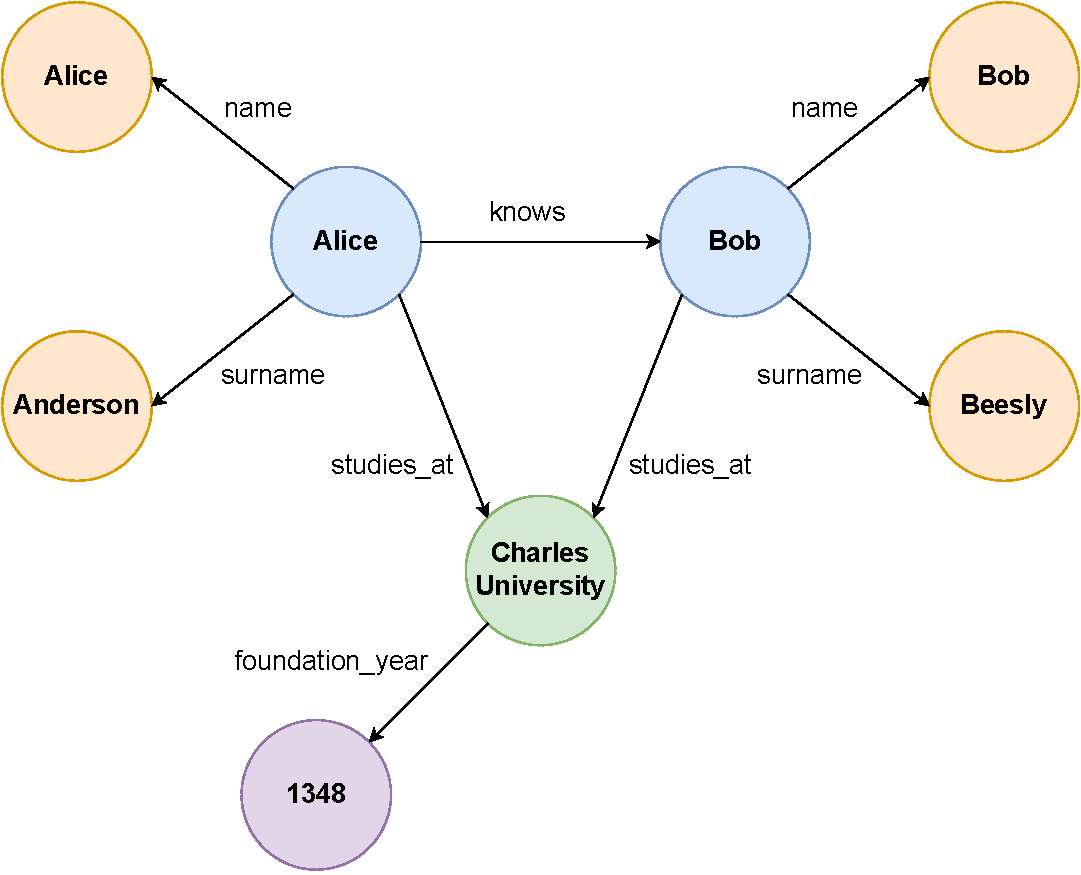
\includegraphics[width=0.8\textwidth]{img/edge-labeled-graph.pdf}}}
\caption{Data modeled as an edge-labeled graph.}
\label{fig:edgegraph}
\end{figure}

Edge-labeled graphs are the data model for the Resource Description Framework~(RDF)~\cite{rdf}, for which SPARQL~\cite{sparql} acts as the most popular query language.
RDF is a framework for representing information on the Web, and it models information as triples in the form \textit{subject predicate object}.
RDF graphs may contain three types of nodes: Internationalized Resource Identifiers~(IRIs), literals (value types like strings and numbers) and blank nodes (vertices without a globally persistent IRI).
Predicates are always IRIs, which can be equated to edges with labels from edge-labeled graphs.

\subsection{Property Graphs}

A graph data model used more widely in practice by graph-oriented databases is the property graph.
A property graph can be seen as an extension of edge-labeled graphs, where both vertices and edges may be labeled.
In addition, each vertex and edge may be associated with a set of key-value pairs called \textit{attributes}, which store additional information about the vertex or edge.
An example of data modeled as a property graph can be seen in~\cref{fig:propgraph}.

\begin{figure}[ht]
\centerline{\mbox{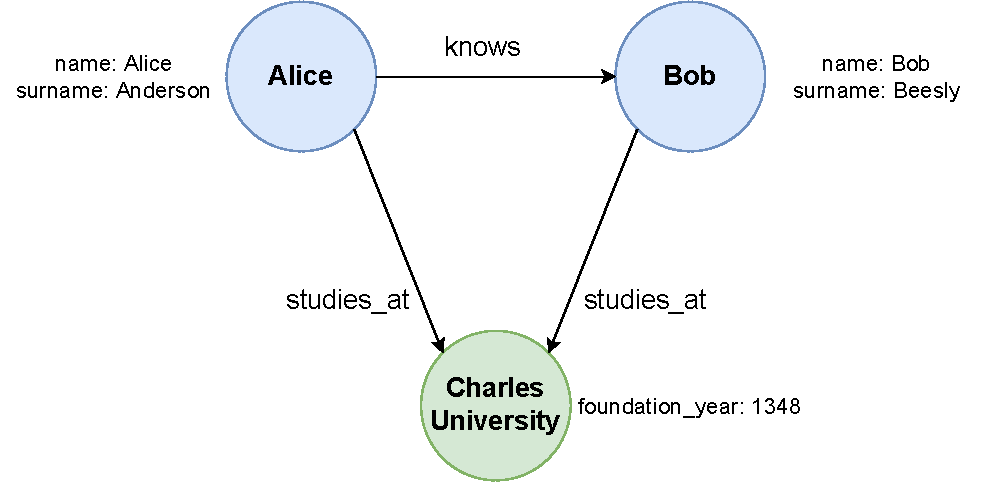
\includegraphics[width=0.8\textwidth]{img/property-graph.pdf}}}
\caption{Data modeled as a property graph.}
\label{fig:propgraph}
\end{figure}

These additional constructs do not give property graphs a higher expressive power compared to edge-labeled graphs, but they do carry other benefits.
First of all, the structure of the data in property graphs may be easier for users to work with, since data related to a particular vertex or edge is associated directly with that vertex or edge, rather than residing in a different vertex.
Additionally, imagine a scenario where we have an edge-labeled graph, and we need to add a property to an edge which previously did not have any properties.
The solution to this problem is to use reification and create a new in-between vertex holding the new property.
However, such a change is disruptive to the schema of the data, and will necessarily break existing queries.
Using the property graph model, such a change can be done without significantly disrupting the schema.

The property graph  model forms the basis for the majority of modern graph data platforms.
The foremost among them are Neo4j\footnote{\url{https://neo4j.com/}} and Apache TinkerPop\footnote{\url{https://tinkerpop.apache.org/}}, which primarily allow querying with Cypher~\cite{opencypher} and Gremlin~\cite{gremlin} respectively.

\section{Language Features}

With the graph data models clarified, we analyze the specifics of each selected graph query language.
The presented languages are a sample of the most popular graph query languages which cover a variety of concepts and problem domains.
% Maybe I should write another paragraph about the most important features and their explanations? Something like 'joins and unions and projections exist, what is composability etc
Specifically, this section focuses on the querying capabilities of the given languages, and only briefly covers their mutation functionality.

\subsection{SPARQL}
\label{querylanguages:subsection:sparql}

As SPARQL~\cite{sparql} is primarily used as the query language for RDF~\cite{rdf}, it is different from the other selected query languages in that it operates on an edge-labeled graph.
It operates in terms of triple patterns~--~whitespace-separated lists consisting of a subject, predicate, and object.
Any part of the triple pattern may consist of a constant (IRI or RDF literals like strings and numbers) or a variable.
These triple patterns can then be used to match parts of the queried graph.
SPARQL itself only supports querying, but SPARQL 1.1 Update~\cite{sparql_update}, which is an update language for RDF graphs, allows for updates with a syntax very similar to SPARQL.

\begin{figure}[ht]
\begin{code}[]
PREFIX lib: <http://example.org/library#>

SELECT ?author ?book
WHERE
{
    ?author lib:authored    ?book .
    ?book   lib:releaseYear 2015  .
    ?author lib:birthYear   ?authorBirthYear .
}
ORDER BY ASC(?authorBirthYear)
\end{code}
\caption{Basic SPARQL query example.}
\label{fig:sparqlbasic}
\end{figure}

A simple SPARQL query which retrieves a list of books released in 2015 and their respective authors (ordered by birth year) may be seen in \Cref{fig:sparqlbasic}.
It can be seen that the SPARQL query structure is in some ways inspired by SQL~--~we have a \texttt{SELECT} clause specifying what the query should return, as well as a \texttt{WHERE} clause specifying the conditions for the returned variables, and an \texttt{ORDER BY} clause.
However, these similarities end upon inspection of the graph querying capabilities of SPARQL.
In order for a set of variable bindings to be returned by the query, their substitution into the \texttt{WHERE} clause must induce a valid subgraph of the queried graph.
This \texttt{WHERE} clause utilizes the aforementioned triple patterns to this end.
In the sample query, the first triple pattern specifies that the query should match triples in the form of \texttt{?author lib:authored ?book .}, where the dot at the end signifies the end of the triple.
The second triple specifies that the matched book should be released in 2015.
Specifying both triples after one another in the \texttt{WHERE} clause functions as their conjunction - both must match in order for the entire \texttt{WHERE} clause to match.
Lastly, the \texttt{PREFIX} clause simply specifies the prefix \texttt{lib:} to be equivalent to the namespace IRI \texttt{http://example.org/library\#}.
This does not increase the expressive power of SPARQL, but it makes queries significantly more readable compared to queries which use the full namespace IRI at every occurrence.

SPARQL also supports more complex graph patterns such as joins, unions, differences, optional matching, and filtering.
Joins are implicit both between triple patterns and graph patterns -- they act as a natural join on the set of shared variables between the two patterns whenever they are specified within the same graph pattern.
The \texttt{MINUS} and \texttt{NOT EXISTS} expressions allow the elimination of matches depending on the evaluation of a pattern and the existence of a pattern respectively.
Using the \texttt{OPTIONAL} keyword, the query may specify that parts of the graph pattern are optional, meaning that when they cannot be successfully matched for a given solution, that solution is not discarded, but rather any unmatched variables remain unbound.
Filtering matches are possible using the \texttt{FILTER} keyword, which specifies a condition and filters all matches which do not satisfy this condition.

\begin{figure}[ht]
\begin{code}[]
PREFIX lib: <http://example.org/library#>

SELECT ?author ?book ?rating
WHERE
{
    { ?author lib:authored ?book . }
    UNION
    { ?author lib:coauthored ?book .}
    
    ?book   lib:releaseYear ?releaseYear .
    OPTIONAL { ?book lib:rating ?rating . }
    
    FILTER(?releaseYear >= 2015)
}
\end{code}
\caption{More complex graph pattern matching in a SPARQL query.}
\label{fig:sparqlpattern}
\end{figure}

More complex graph pattern matching can be seen in \Cref{fig:sparqlpattern}.
This query returns the list of authors and co-authors of books which have been released in  2015 or later, and additionally returns the book rating if it is available.
If the rating is not present in the data, that book is still returned, with the \texttt{?rating} variable remaining unbound.
The \texttt{UNION} construct in the query ensures that results will be returned for both authors and co-authors of any given book.

When it comes to navigational queries (i.e. queries which navigate the graph), SPARQL uses the concept of \textit{property paths}.
These are constructs not unlike regular expressions, which specify possible routes through a graph between two graph nodes.
Property paths may contain RDF terms or variables at both ends, but they cannot contain variables as part of the path itself.
An example of a property path is \texttt{lib:TheHobbit lib:sequel+ ?book .}, which will bind the \texttt{?book} variable to any book which follows The Hobbit as a direct or indirect sequel.
A path like \texttt{lib:TheHobbit lib:sequel/lib:rating ?rating .} would bind \texttt{?rating} to the rating of The Hobbit's direct sequel.
Additional property path features include inverse paths from object to subject, alternative paths or negated property sets which match any except the specified IRIs in the path.

\Cref{fig:sparqlnav} shows a query which returns the list of all authors who co-authored a book with J. R. R. Tolkien.
This query uses a property path to find all books co-authored by Tolkien, and then uses an inverse path from these books to their co-authors.
Note that it is necessary to filter Tolkien himself from the results of the query, as the \texttt{?author} variable would otherwise match Tolkien himself, as he is naturally a co-author for all books he co-authored.

\begin{figure}[ht]
\begin{code}[]
PREFIX lib: <http://example.org/library#>

SELECT DISTINCT ?author
WHERE
{
    lib:JRRTolkien lib:coauthored/^lib:coauthored ?author .
    FILTER(?author != lib:JRRTolkien) .
}
\end{code}
\caption{Graph navigation in a SPARQL query.}
\label{fig:sparqlnav}
\end{figure}

SPARQL is most notably supported by the Virtuoso\footnote{\url{https://virtuoso.openlinksw.com/}}, Amazon Neptune\footnote{\url{https://aws.amazon.com/neptune/}}, Stardog\footnote{\url{https://www.stardog.com/}}, Apache Jena Fuseki\footnote{\url{https://jena.apache.org/documentation/fuseki2/}} or GraphDB\footnote{\url{https://graphdb.ontotext.com/}} graph databases.

\subsection{Cypher}

Cypher~\cite{opencypher} is a declarative graph query language originally developed by Neo4j.
It was open-sourced in 2015 and contributed to the openCypher~\cite{opencypher} project, which is now responsible for maintaining the language.
Cypher operates on a property graph data model, referring to the vertices of the graph as \textit{nodes} and the edges as \textit{relationships}.
Its structure is inspired by SQL, as queries are composed of various clauses.
Its pattern matching is also inspired by SPARQL~\cite{sparql}.
Cypher may be used for both querying and updating graphs.

Clauses in a Cypher query are chained together, and the results of each clause become the inputs for the next clause.
Regarding basic graph pattern matching, Cypher notation tries to be very intuitive when it comes to the underlying graph data model.
It models relationships as an arrow between two nodes: \texttt{(a)-[r]->(b)}.
Such a pattern describes a directed relationship \texttt{r} from the node \texttt{a} to the node \texttt{b}.
Note that both nodes and relationships do not have to be named, they may simply use the \texttt{()} and \texttt{[]} notation respectively.
The pattern \texttt{(a)-[]-(b)} will match the relationship in either direction.
These patterns are used in the \texttt{MATCH} clause, which matches the patterns to the underlying data and binds any variables accordingly.

It should be noted that unlike SPARQL, Cypher does not return matches where the same graph relationship is found multiple times in a single pattern.
What this means is that if we specify a pattern like \texttt{(a)-[]->(b)<-[]-(c)}, Cypher implicitly makes sure that the node \texttt{a} is distinct from the node \texttt{c}.
If allowing the return of the same node in different parts of the pattern is desirable, multiple consecutive \texttt{MATCH} clauses must be used, matching parts of the pattern separately and using some common variables to join them together.

\begin{figure}[ht]
\begin{code}[]
MATCH (author:Author) -[:AUTHORED]-> (book:Book {releaseYear: 2015})
RETURN author, book
ORDER BY author.birthYear ASC
\end{code}
\caption{Basic Cypher query example.}
\label{fig:cypherbasic}
\end{figure}

The last information needed for composing a simple query is knowing how to specify labels and properties.
The construct \texttt{(a:Author {surname: "Tolkien"})} \texttt{-[r:AUTHORED]->} \texttt{(b)} will match \texttt{a} to nodes labeled \texttt{Author} and with the property \texttt{surname} equal to "Tolkien", and \texttt{r} to relationships typed \texttt{AUTHORED}.
The query shown in \Cref{fig:cypherbasic} uses these principles to return a list of books released in 2015 and their respective authors (ordered by birth year).
The \texttt{RETURN} clause is used for projection on the output variables, and it is mandatory in queries which do not mutate the underlying dataset.
The \texttt{ORDER BY} clause works similarly to SQL.

Much like SPARQL pattern matching, joins happen implicitly when we specify multiple \texttt{MATCH} clauses in succession.
The \texttt{NOT} operator acts as a difference -- its usage in a \texttt{WHERE} clause after a \texttt{MATCH} clause will eliminate matching results from the results of the \texttt{MATCH} clause.
Optional pattern matching is also supported with the \texttt{OPTIONAL MATCH} clause.
Filtering is accomplished with the \texttt{WHERE} clause.

\begin{figure}[ht]
\begin{code}[]
MATCH (author:Author) -[:AUTHORED]-> (book:Book)
OPTIONAL MATCH (book) -[:RATING]-> (rating:Rating)
WHERE book.releaseYear >= 2015
RETURN author, book, rating.average AS rating

UNION

MATCH (author:Author) -[:COAUTHORED]-> (book:Book)
OPTIONAL MATCH (book) -[:RATING]-> (rating:Rating)
WHERE book.releaseYear >= 2015
RETURN author, book, rating.average AS rating
\end{code}
\caption{More complex graph pattern matching in a Cypher query.}
\label{fig:cypherpattern}
\end{figure}

\Cref{fig:cypherpattern} shows a more complex example of graph pattern matching using some of the features mentioned above.
The depicted query returns the list of authors and co-authors of books released in the year 2015 or later, and additionally returns the book rating if it is available (for simplicity's sake, we assume that the rating is stored in a node connected to a book via the \texttt{RATING} relationship).
It should be noted that Cypher does not have an easy way of specifying alternate matches like SPARQL does, and the \texttt{UNION} clause works at the level of query results.
Therefore we need to run both queries independently, and then \texttt{UNION} their results.
Cypher also does not yet support post-union processing, so if we wanted to order the results of the union, we would need to resort to other workarounds.

As far as navigational queries go, the strength of Cypher is considerably lower than that of SPARQL.
Traversal of a path is limited to a single relationship type (i.e. label), and if multiple labels are desired, the traversal has to be broken up into multiple parts.
The same applies to properties of the relationship -- path pattern matching is only able to match the same set of properties and property values for each relationship in the path.
Variable-length pattern matching is signified by the usage of the \texttt{*} operator.
The pattern \texttt{(a)-[*2]->(b)} is equivalent to the pattern \texttt{(a)-[]->()-[]->(b)},
i.e. a path of length 2.
The length of this path can be variable: \texttt{(a)-[*2..4]->(b)} means that the path is at least of length 2 but no more than length 4.
Either of these bounds can be omitted, meaning \textit{length X or more} or \textit{length X or less}.
If both bounds are omitted, the path can be of any length: \texttt{(a)-[*]->(b)}, as the lower and upper bounds default to 1 and infinity respectively.
The ability to specify a range for the path length present in Cypher is not present in SPARQL.

What Cypher lacks in terms of path traversal specification, it makes up for in other ways of working with paths.
It features paths as a first-class citizen of the language, offering the ability to save paths to variables or to return them from queries.
It also has a number of interesting functions like searching for one or all shortest paths between two nodes in the graph.
Cypher also has native support for list primitives, something which is missing from SPARQL (and RDF).

\begin{figure}[ht]
\begin{code}[]
MATCH path = (:Book {title: "The Hobbit"}) -[*:SEQUEL]-> (book:Book)
RETURN book.title AS title, length(path) + 1 AS seriesNumber
\end{code}
\caption{Graph navigation in a Cypher query.}
\label{fig:cyphernav}
\end{figure}

\Cref{fig:cyphernav} demonstrates a query which returns the list of all sequels of the book The Hobbit transitively.
The query also returns for each book its number in the series, meaning The Hobbit's direct sequel will have the number 2, its sequel the number 3 and so on.

The most notable databases using Cypher are Neo4j\footnote{\url{https://neo4j.com/}}, Amazon Neptune\footnote{\url{https://aws.amazon.com/neptune/}}, Memgraph\footnote{\url{https://memgraph.com/}}, Katana Graph\footnote{\url{https://katanagraph.com/}} and RedisGraph\footnote{\url{https://redis.io/docs/stack/graph/}}.

\subsection{Gremlin}

Gremlin~\cite{gremlin} is a graph traversal language operating on property graphs.
It was developed by Apache TinkerPop of the Apache Software Foundation, and is available under the Apache License 2.0.
Gremlin is a functional language which operates in terms of a data flow.
A traversal in Gremlin consists of a sequence of steps, each of which performs an operation on the underlying stream of data.
This data is functionally passed between three kinds of steps: map steps which transform the data, filter steps which filter, and remove some of the data, and side effect steps which can compute statistics about the data stream.

\begin{figure}[ht]
\begin{code}[]
g.V().
    hasLabel('Book').
    has('releaseYear', 2015).
    as('book').
    
    in('authored').

    hasLabel('Author').
    as('author').

    select('book', 'author').
        by('title').
        by('name')
\end{code}
\caption{Basic Gremlin query example with imperative traversal.}
\label{fig:gremlinbasic}
\end{figure}

\Cref{fig:gremlinbasic} shows a simple Gremlin query which retrieves the list of books released in 2015 and their respective authors, returning their titles and names.
The \texttt{g.V()} step returns a list of all vertices in the graph.
Using \texttt{hasLabel('Book')}, only vertices with the Book label are selected.
Similarly, the \texttt{has()} step filters out books which were not released in 2015.
The \texttt{as()} step is not a real step, but rather a step modulator which assigns a label to the previous step, making it accessible by later steps.
It can be thought of as referencing to that step with a variable.
Edge traversal is performed with the \texttt{in()} step, which in the example traverses incoming edges with the \texttt{authored} label.
Other edge traversal steps exist which traverse edges in a specified direction, or both.
The \texttt{select()} step takes data from previously labeled steps and collects them, additionally projecting the data to the book title and author name.

Gremlin differs from the previously mentioned graph query languages by allowing imperative graph traversal as shown in \Cref{fig:gremlinbasic}, but it also supports declarative traversals, as well as allowing mixing of imperative and declarative traversals.
An example of a declarative traversal can be seen in \Cref{fig:gremlinpattern}.
While declarative pattern matching is possible, it is considerably less succinct than its SPARQL or Cypher equivalents, as Gremlin focuses primarily on graph traversal.
Gremlin also supports filtering and unions, but other more complex operation like set differences and optional matching require extra effort.

\begin{figure}[ht]
\begin{code}[]
g.V().
    match(
        as('tolkien').
            hasLabel('Author').
            has('name', 'J. R. R. Tolkien'),
        as('tolkien').
            out('coauthored').
            as('book'),
        as('book').
            in('coauthored').
            as('coauthor'),
        where('coauthor', neq('tolkien'))
    ).
    select('coauthor').by('name')
\end{code}
\caption{Declarative graph pattern matching in a Gremlin query.}
\label{fig:gremlinpattern}
\end{figure}

Gremlin supports variable-length paths via the \texttt{repeat()} step, which offers both do-while and while-do semantics.
The \texttt{repeat()} step may repeat any traversal, meaning the repeated traversal may itself consist of multiple steps.
\Cref{fig:gremlinnav} showcases this in a query which performs a full traversal of the graph by iteratively following edges.
This traversal starts with the author J. R. R. Tolkien, and follows outgoing edges until it gets to end nodes which have no outgoing edges.
It uses the \texttt{simplePath()} step to eliminate any potential cycles in the graph during traversal.
It also contains another stop condition -- the maximum traversal depth of 10 set with \texttt{loops().is(10)}.
Gremlin is also able to return entire paths from a query.

\begin{figure}[ht]
\begin{code}[]
g.V().
    hasLabel('Author').
    has('name', 'J. R. R. Tolkien').
    
    repeat(out().simplePath()).
        until(outE().count().is(0).
            or().loops().is(10))
\end{code}
\caption{Graph navigation in a Gremlin query.}
\label{fig:gremlinnav}
\end{figure}

Gremlin can be used for both Online Transaction Processing (OLTP) and Online Analytical Processing (OLAP), meaning a Gremlin traversal can be executed as either a real-time database query, or as a batch analytics query.
Notable graph databases implementing Gremlin are Amazon Neptune\footnote{\url{https://aws.amazon.com/neptune/}}, OrientDB\footnote{\url{https://orientdb.org/}}, Blazegraph\footnote{\url{https://blazegraph.com/}} and Titan\footnote{\url{https://titan.thinkaurelius.com/}}.
